\section{Экспериментальные методы}

Для оценки достоверности разработанной модели СЭЛТР должна быть проведена ее верификация на основе профилей, полученных экспериментально. В этом разделе описаны подходы, применявшиеся при формировании структур методом СЭЛТР и получении профилей этих структур.

\subsection*{Растровая электронная микроскопия}

В растровой электронной микроскопии (РЭМ) изображение объекта формируется последовательно по точкам, каждая из которых получается за счет облучения поверхности объекта сфокусированным электронным пучком.
При взаимодействии первичных электронов с веществом возникают вторичные сигналы различной физической природы -- отраженные и вторичные электроны, Оже-электроны, рентгеновское излучение и пр. (рисунок~\ref{fig:REM_1}).
Величины вторичных сигналов зависят от физических свойств поверхности исследуемого образца и могут изменяться от точки к точке.
Регистрация вторичных сигналов соответствующими детекторами позволяет сформировать на экране монитора изображение поверхности образца, отображающее топографию какого-либо его физического свойства.
За счет этого можно исследовать форму поверхности образца -- в обратно отраженных или вторичных электронах; распределение элементного состава по поверхности образца -- в характеристическом рентгеновском излучении; распределение донорных или акцепторных центров -- по величине поглощенного тока и т. д.

\begin{figure}
	\centering
	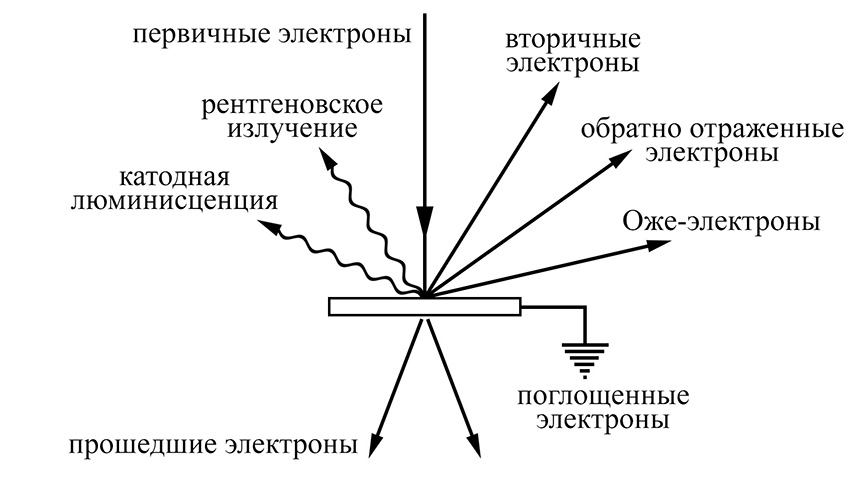
\includegraphics[width=0.9\textwidth]{experiment/REM_1_small}
	\caption{Схема образования вторичных сигналов при взаимодействии электронного пучка с веществом мишени.}
	\label{fig:REM_1}
\end{figure}

%При нормальном атмосферном давлении электронный пучок сильно рассеивается и поглощается, что делает невозможным его фокусировку.
%В силу этого давление в камере растрового электронного микроскопа должно составлять порядка 10$^\text{-5}$ торр или ниже.
Схема основных элементов растрового электронного микроскопа приведена на рисунке~\ref{fig:REM_2}.
Электронный пучок формируется электронно-оптической системой и проходит через систему управляющих электродов или электромагнитов, которые перемещают пятно пучка по поверхности образца, образуя растр.
Электронно-оптическая система включает в себя источник электронов (вольфрамовый катод, катод из гексаборида лантана или автоэмиссионный катод), модулятор (цилиндра Венельта) и анод (рисунок~\ref{fig:REM_3}).

\begin{figure}[t]
	\centering
	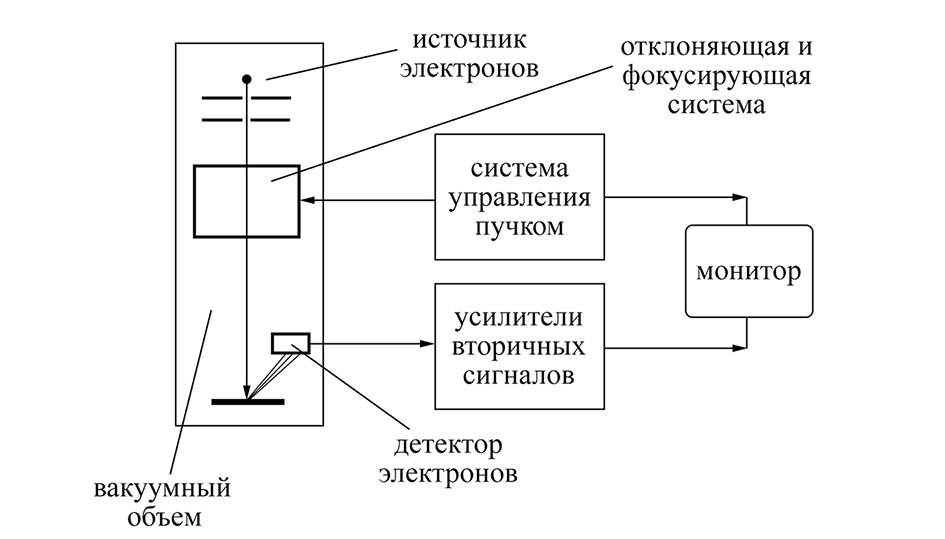
\includegraphics[width=0.95\textwidth]{experiment/REM_2_200}
	\vspace{0.5em}
	\caption{Упрощенная схема, иллюстрирующая работу РЭМ.}
	\label{fig:REM_2}
\end{figure}

\begin{figure}[h]
	\centering
	\includegraphics[width=0.75\textwidth]{experiment/REM_3_200_large}
	\vspace{0.5em}
	\caption{Схема устройства электронно-оптической системы растрового электронного микроскопа.}
	\label{fig:REM_3}
\end{figure}

\paragraph{Сцинтилляционный детектор} \mbox{} \\
\indent В настоящее время для регистрации вторичных электронов широко используются сцинтилляционные детекторы.
Вторичные электроны, попадая на сцинтиллятор, генерируют в нем световой импульс, который регистрируется и преобразуется в электрический сигнал с помощью фотоэлектронного умножителя.
Так как большинство используемых сцинтилляторов генерируют свет под действием электронов с энергией более 10~кэВ, на внешнюю поверхность сцинтиллятора наносится тонкий металлический слой, и на него подается положительное напряжение (порядка 10 кВ) для сбора и ускорения низкоэнергетической части спектра вторичных электронов.

\paragraph{Полупроводниковый детектор} \mbox{} \\
\indent Вторичные электроны, попадающие в полупроводник вблизи \textit{p-n}-перехода, создают в нем электронно-дырочные пары, что приводит к появлению тока через \textit{p-n}-переход.
Для получения сигнала достаточной величины этот ток в дальнейшем усиливается специальными малошумящими усилителями.
Электроны должны иметь энергию, достаточную для образования электронно-дырочных пар, поэтому полупроводниковый детектор обычно используется для регистрации высокоэнергетической части спектра вторичных электронов.

\paragraph{Детектор излучения катодолюминесценции} \mbox{} \\
\indent Количество света, испускаемого мишенью под воздействием электронного пучка, обычно мало, поэтому для увеличения эффективности регистрации испускаемого света используют специальные эллиптические зеркала. В один из фокусов зеркала помещают мишень, а в другой -- световод-приемник, уводящий свет за пределы вакуумной камеры микроскопа. Далее свет регистрируется фотоэлектронным умножителем или спектрометром.

\paragraph{Детекторы рентгеновского излучения} \mbox{} \\
\indent Для регистрации рентгеновского излучения используются два типа систем. Во-первых, применяются кристалл-дифракционные спектрометры с изогнутыми для увеличения светосилы кристаллами-анализаторами.
Приемником рентгеновского излучения в них обычно служит сцинтилляционный детектор.
В качестве кристалла-сцинтиллятора обычно используются монокристаллы NaI(Tl).
Во-вторых, применяются энергодисперсионные системы, например, кремний-литиевые детекторы.
Энергодисперсионные детекторы имеют существенно более низкое энергетическое разрешение (100--150 эВ) по сравнению с кристалл-дифракционными спектрометрами (менее 10 эВ), однако они получили широкое распространение благодаря возможности регистрации всего спектра вторичных электронов без каких-либо перемещений образца и детектора, а также возможности быстрой обработки спектра на ЭВМ.


\subsection*{Атомно-силовая микроскопия}

Принцип работы атомно-силового микроскопа (АСМ) основан на силовом взаимодействии между сторонним телом и поверхностью образца, для регистрации которого используются специальные датчики, представляющие собой упругую консоль (кантилевер) с острым зондом на конце (рисунок~\ref{fig:AFM_1_2}а).
%Сила, действующая на зонд со стороны поверхности, приводит к изгибу кантилевера, и за счет регистрации величины изгиба в разных точках сканируемой поверхности можно определить профиль поверхности.
Взаимодействие между зондом и поверхностью образца, можно описать на примере двух атомов, энергия взаимодействия которых аппроксимируется потенциалом Леннард-Джонса (рисунок ~\ref{fig:AFM_1_2}б):
\begin{equation}
	U_\mathrm{LJ}(r) = U_0\left\{ -2\left(\frac{r_0}{r}\right)^6 + \left(\frac{r_0}{r}\right)^{12}\right\},
\end{equation}
где $r_0$ -- равновесное расстояние между атомами, $U_0$ -- глубина потенциальной ямы.
Первое слагаемое в скобках описывает дальнодействующее притяжение, обусловленное диполь-дипольным взаимодействием атомов, второе -- отталкивание на малых расстояниях за счет обменного взаимодействия.
Взаимодействие зонда с образцом имеет сложный характер, однако основные свойства взаимодействия, характерного для двух атомов, сохраняются -- зонд АСМ испытывает притяжение со стороны образца на больших расстояниях от его поверхности и отталкивание -- на малых.

\begin{figure}[b]
	\centering
	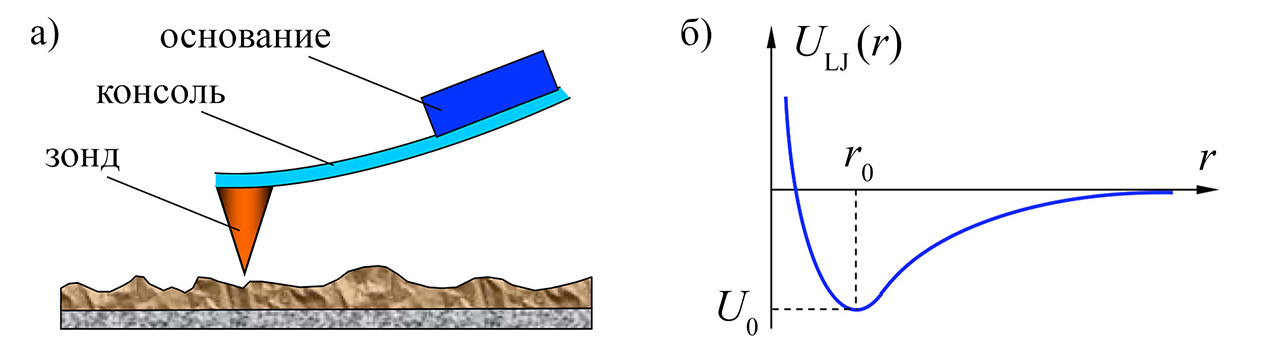
\includegraphics[width=0.9\textwidth]{experiment/AFM_1_2_200}
	\vspace{0.5em}
	\caption{Схематическое изображение зондового датчика АСМ (а) и качественный вид потенциала Леннард-Джонса (б).}
	\label{fig:AFM_1_2}
\end{figure}

Получение изображения рельефа поверхности с помощью АСМ связано с регистрацией малых изгибов кантилевера, для чего используется следующая оптическая схема: луч лазера направляется на внешнюю поверхность кантилевера, отражается и попадает в центр четырехсекционного полупроводникового фотодиода (рисунок~\ref{fig:AFM_2}).

\begin{figure}[h]
	\centering
	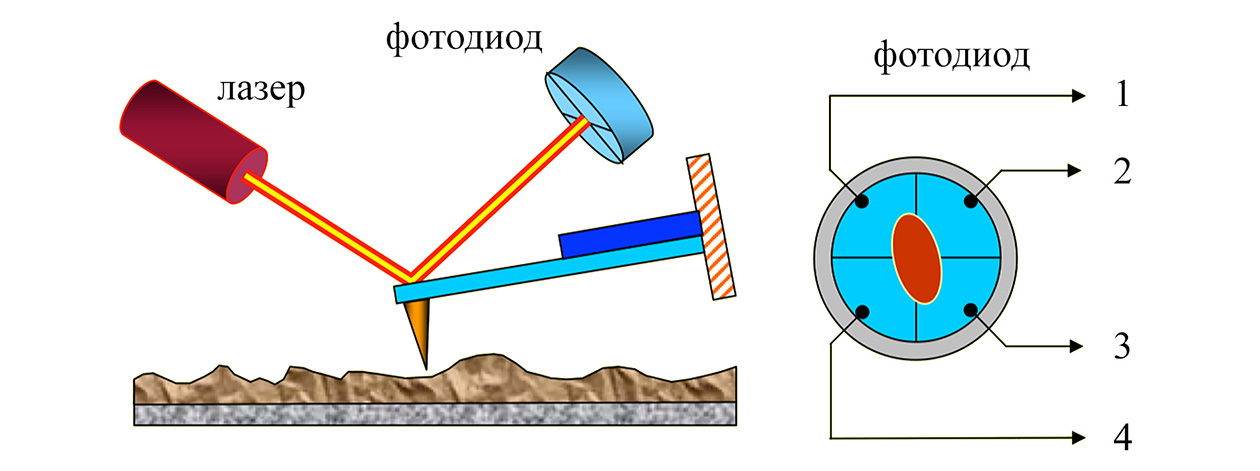
\includegraphics[width=0.9\textwidth]{experiment/AFM_3_200}
	\vspace{0.2em}
	\caption{Схема оптической регистрации изгиба кантилевера АСМ.}
	\label{fig:AFM_2}
\end{figure}

Основные регистрируемые оптической системой параметры -- это деформации изгиба консоли под действием $Z$-компонент сил притяжения или отталкивания ($F_\mathrm{Z}$) и деформации кручения консоли под действием латеральных компонент сил ($F_\mathrm{L}$) взаимодействия зонда с поверхностью. Если обозначить исходные значения фототока в секциях фотодиода через $I_{01}$, $I_{02}$, $I_{03}$, $I_{04}$, а через $I_{1}$, $I_{2}$, $I_{3}$, $I_{4}$ -- значения токов после изменения положения консоли, то разностные токи в различных секциях фотодиода $\Delta I_i = I_i - I_{0i}$ будут однозначно характеризовать величину и направление изгиба консоли зондового датчика АСМ. Действительно, комбинация разностных токов вида
\begin{equation}
	\Delta I_\mathrm{Z} = \left(\Delta I_1+\Delta I_2\right)-\left(\Delta I_3+\Delta I_4\right)
\end{equation}
пропорциональна изгибу консоли под действием силы, действующей по нормали к поверхности образца, а комбинация вида
\begin{equation}
	\Delta I_\mathrm{L} = \left(\Delta I_1+\Delta I_4\right)-\left(\Delta I_2+\Delta I_3\right)
\end{equation}
характеризует изгиб консоли под действием латеральных сил.

Величина $\Delta I_\mathrm{Z}$ используется в качестве входного параметра в петле обратной связи атомно-силового микроскопа.
Система обратной связи обеспечивает постоянное значение $\Delta I_\mathrm{Z}$ с помощью пьезоэлектрического исполнительного элемента, который поддерживает изгиб консоли $\Delta Z$ равным величине $\Delta Z_0$, задаваемой оператором.
При сканировании образца в режиме $\Delta Z = const$ зонд перемещается вдоль поверхности, при этом напряжение на $Z$-электроде сканера записывается в память компьютера, что позволяет впоследствии воспроизвести рельеф поверхности.
Пространственное разрешение АСМ определяется радиусом закругления зонда и чувствительностью системы, регистрирующей отклонения консоли.
В настоящее время реализованы конструкции АСМ, позволяющие исследовать поверхность образцов с атомарным разрешением.
